\newpage
\section{Un système de commits}

Git fonctionne un peu comme svn : par un système de version, ici appelés commit.\\
Pour commencer : créez un fichier nommé yoyo.txt et écrivez "Version 1" dedans.

A ce moment précis, vous considérez avoir bien travaillé et souhaitez \textbf{sauvegarder} votre travail dans git, de manière à le retrouver si jamais, plus tard, le fichier aurait un problème.

Nous allons donc créer une nouvelle version du projet.

\subsection{Indexer les fichiers}
Avant de créer un commit, nous devons dire à git quels fichiers doivent être pris en compte :
on appelle ça indexer les fichiers.
Indexer un fichier le mettra directement en cache, dans le dépôt.

\textbf{Attention : } Seuls les fichiers normaux et leur chemin sont mis en cache. Git en prend pas en compte les dossiers.\\
Si git veut nous créer un fichier sur notre ordinateur, si le dossier n'existe pas, il le fabrique.\\
Si on veut indexer un dossier vide, rien ne se passera.

\subsubsection{Par ligne de commande}
\begin{verbatim}
# Indexer le fichier1, le fichier2, et tous les fichiers du dossier3 (récursif)
$ git add <fichier1> [fichier2] [dossier3]

# Par exemple : indexe tous les fichier du dossier courant (et les ajoute au cache)
$ git add .

# Pour savoir quels sont les fichiers ajoutés, à ajouter, 
# modifiés (comparé au commit précédent)
$ git status
\end{verbatim}

Pour désindexer un fichier (supprimer le fichier et arrêter sa sauvegarde par le système de fichier), vous devrez passer par la commande git rm ou bien en supprimant au préalable le fichier et en utilisant l'option -A avec la commande git add.\\

Si vous souhaitez conserver le fichier dans votre système mais le retirer de l'index de git, il faut utiliser la commande git rm --cached

\subsubsection{Avec tortoise git}
Clic droit $\rightarrow$ Tortoise Git $\rightarrow$ Add

Tortoise git aide à l'indexation pendant le commit, il vous est en soi inutile de faire Add.\\
\newpage
\subsection{Créer un commit}
\subsubsection{Par ligne de commande}
\begin{verbatim}
# Créer un commit
$ git commit
\end{verbatim}

\textbf{Attention : } Vous allez entrer en mode texte (programme Vi) pour insérer un message.
Ici les lignes commançant par \# seront ignorées.
Pour éditer le texte, appuyez sur "i", pour arrêter l'édition, appuyez sur "Echap", pour valider le message :
arrêtez l'édition puis tapez ":wq"\\

Pour éviter de rentrer dans ce mode texte, vous pouvez écrire le message dans la commande :
\begin{verbatim}
# Créer un commit et tapez directement son message
$ git commit -m "Message"
\end{verbatim}

Pour indexer tous les fichiers qui ont été mis en cache :
\begin{verbatim}
# Créer un commit en indexant tous les fichiers mis en cache
$ git commit -a
\end{verbatim}

Vous pouvez aussi bien mélanger les options :
\begin{verbatim}
# Créer un commit en indexant tous les fichiers mis en cache
# et tapez directement son message
$ git commit -a -m "Message"
\end{verbatim}

\subsubsection{Par tortoise git}

Clic droit $\rightarrow$ Git Commit $\rightarrow$ "master"\\

Une fenêtre doit s'ouvrir contenant :
\begin{itemize}
\item Les fichiers mis en cache (avec une case cochée)
\item Les fichier non indexés (avec une case décochée)\\
\end{itemize}

La case indique s'il faut indexer ou non le fichier pour le commit à venir.
Si le fichier n'était pas en cache, il sera ajouté au dépôt et mis en cache\\

Une fois les fichiers choisis : tapez le message du commit (tentez d'être clair), signez, puis validez.\\

Vous pouvez aussi le faire directement depuis le log en faisant:
Clic droit $\rightarrow$ Tortoise git $\rightarrow$ Show log\\

Vous y verrez vos commits et les modifications courantes.\\
Pour créer un commit à partir de là : Clic droit sur "Working dir changes" $\rightarrow$ Commit
\newpage
\paragraph{Fenêtre de commit } Ici, le fichier toto.txt à été modifié, et le fichier nouveau.txt à été crée sans avoir encore été mis en cache/indexé.

\begin{figure}[h] 
	\begin{center}
		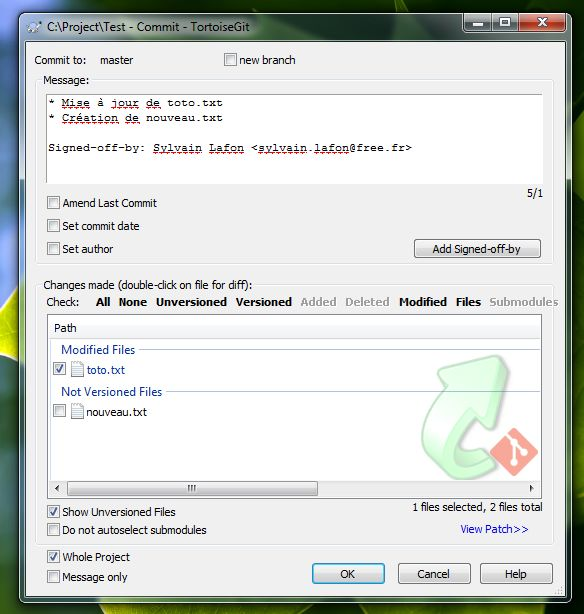
\includegraphics[scale=0.3]{../IMG/commit.jpg}
	\end{center}
	\caption{Tortoise Git : fenetre de commit}
	\label{Tortoise Git : fenetre de commit} 
\end{figure}

Pour ajouter le fichier nouveau, il suffit de cliquer sur la case à sa gauche.\\

\paragraph{Le log } Voici ce dont à quoi ressemble la fenêtre de log :

\begin{figure}[h] 
	\begin{center}
		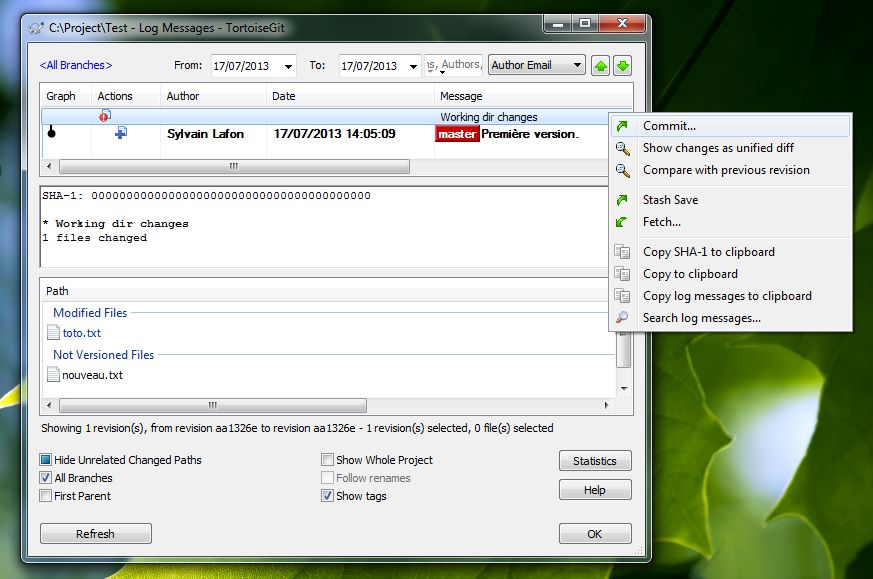
\includegraphics[scale=0.3]{../IMG/log.jpg}
	\end{center}
	\caption{Tortoise Git : fenetre de log}
	\label{Tortoise Git : fenetre de log} 
\end{figure}

Cette fenêtre doit être la fenêtre la plus importante de Tortoise git : elle permet d'afficher les commits en faisant leur graphe à leur gauche, en permettant, au clic droit de faire toutes les opérations que l'on verra.\\
Ici, un clic droit sur "Working dir. changes" permet de créer un commit,
on peut aussi faire des clics droit sur les branches, tags et commits.
\newpage
\subsection{Bien nommer les commits}

Idéalement, un commit devrait se présenter sous la forme suivante :
La première ligne devrait comporter moins de 50 caractères et résume les changements du commit.
Elle devrait être suivie d'une ligne blanche, puis des lignes qui décrivent plus en détail les différentes modifications.\\

Le texte situé au dessus de la ligne blanche est pris comme étant le titre du commit, utilisé dans git. (et Tortoise Git).\\
La commande git format-patch permet par exemple d'envoyer un commit par email et utilise le titre pour le sujet et le reste dans le corps du message.

\subsection{Se déplacer dans les commits}

Pour la suite du tutoriel,
faites deux nouveaux commits en modifiant le contenu de toto.txt

\subsubsection{Par ligne de commande}
\begin{verbatim}
$ git checkout <id>
\end{verbatim}

$<$id$>$ peut être un nom de branche, de tag ou bien l'id (SHA-1) du commit.
Pour connaitre les différents id de commit : 

\begin{verbatim}
$ git log --oneline --color --graph
\end{verbatim}

\subsubsection{Par tortoise git}
Clic droit $\rightarrow$ Tortoise git $\rightarrow$ Switch/Checkout
Une fenêtre apparait pour savoir vers où se déplacer, cochez "Commit" et ouvrez le log, cliquez sur la deuxième version puis "Ok", et "Ok".\\

Votre fichier a dû retrouver le contenu qu'il avait au deuxieme commit.\\

Vous pouvez aussi le faire directement depuis le log en faisant:
Clic droit $\rightarrow$ Tortoise git $\rightarrow$ Show log\\

Puis clic droit sur une version et "Switch/Checkout to this"
La version sur laquelle on se situe sera écrite en gras.
\newpage
\subsection{Référencer les commits importants : les tags}
Vous trouvez que certains commits sont très importants et vous y aimerez y accèder facilement, sans avoir à taper leur SHA-1 ? \\

Pour cela on utilise un tag. Il s'agit d'une simple référence à un commit, un nom.\\

Sur GitHub, une partie "Téléchargement" permet de télécharger le .zip du projet pour chaque tag !

\begin{figure}[h] 
	\begin{center}
		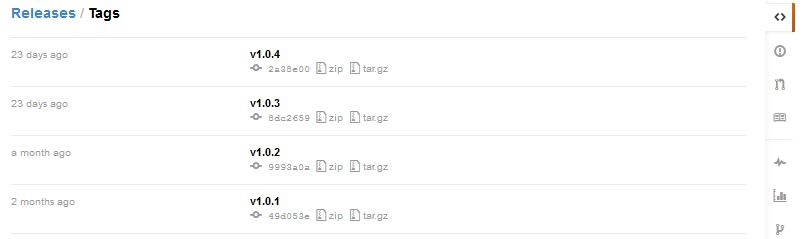
\includegraphics[scale=0.4]{../IMG/tagsdl.jpg}
	\end{center}
	\caption{GitHub : les tags}
	\label{GitHub : les tags} 
\end{figure}

\subsubsection{Par ligne de commande}
Pour commencer, allez sur le commit en question, puis utilisez "git tag"
\begin{verbatim}
# On va sur le commit dont le SHA-1 débute par abcdef
$ git checkout abcdef

# On y crée un tag nommé : "v1.0"
$ git tag v1.0

# On peut désormais y accèder en tapant "v1.0"
$ git checkout v1.0

# Pour SUPPRIMER un tag :
$ git tag -d v1.0
\end{verbatim}

\subsubsection{Par Tortoise Git}
Et par le log et par le menu, on a "Create tag".\\

Pour supprimer un tag, on doit forcément aller dans le log de tortoise git, puis faire un clic-droit sur le tag (en jaune) avant de cliquer sur Supprimer.